\documentclass[paper=letter,11pt]{scrartcl}

\KOMAoptions{headinclude=true, footinclude=false}
\KOMAoptions{DIV=14, BCOR=5mm}
\KOMAoptions{numbers=noendperiod}
\KOMAoptions{parskip=half}
\addtokomafont{disposition}{\rmfamily}
\addtokomafont{part}{\LARGE}
\addtokomafont{descriptionlabel}{\rmfamily}
%\setkomafont{pageheadfoot}{\normalsize\sffamily}
\setkomafont{pagehead}{\normalsize\rmfamily}
%\setkomafont{publishers}{\normalsize\rmfamily}
\setkomafont{caption}{\normalfont\small}
\setcapindent{0pt}
\deffootnote[1em]{1em}{1em}{\textsuperscript{\thefootnotemark}\ }


\usepackage{amsmath}
\usepackage[varg]{txfonts}
\usepackage[T1]{fontenc}
\usepackage{graphicx}
\usepackage{xcolor}
\usepackage[american]{babel}
% hyperref is needed in many places, so include it here
\usepackage{hyperref}

\usepackage{xspace}
\usepackage{multirow}
\usepackage{float}


\usepackage{braket}
\usepackage{bbm}
\usepackage{relsize}
\usepackage{tcolorbox}

\def\ketY{\ensuremath{\ket {\Psi}}}
\def\iGeV{\ensuremath{\textrm{GeV}^{-1}}}
%\def\mp{\ensuremath{m_{\textrm{proton}}}}
\def\rp{\ensuremath{r_{\textrm{proton}}}}
\def\me{\ensuremath{m_{\textrm{electron}}}}
\def\aG{\ensuremath{\alpha_G}}
\def\rAtom{\ensuremath{r_{\textrm{atom}}}}
\def\rNucl{\ensuremath{r_{\textrm{nucleus}}}}
\def\GN{\ensuremath{\textrm{G}_\textrm{N}}}
\def\ketX{\ensuremath{\ket{\vec{x}}}}
\def\ve{\ensuremath{\vec{\epsilon}}}


\def\ABCDMatrix{\ensuremath{\begin{pmatrix} A &  B  \\ C  & D \end{pmatrix}}}
\def\xyprime{\ensuremath{\begin{pmatrix} x' \\ y' \end{pmatrix}}}
\def\xyprimeT{\ensuremath{\begin{pmatrix} x' &  y' \end{pmatrix}}}
\def\xy{\ensuremath{\begin{pmatrix} x \\ y \end{pmatrix}}}
\def\xyT{\ensuremath{\begin{pmatrix} x & y \end{pmatrix}}}

\def\IMatrix{\ensuremath{\begin{pmatrix} 0 &  1  \\ -1  & 0 \end{pmatrix}}}
\def\IBoostMatrix{\ensuremath{\begin{pmatrix} 0 &  1  \\ 1  & 0 \end{pmatrix}}}
\def\JThree{\ensuremath{\begin{pmatrix}    0 & -i & 0  \\ i & 0  & 0 \\ 0 & 0 & 0 \end{pmatrix}}} 
\def\JTwo{\ensuremath{\begin{bmatrix}    0 & 0 & -i  \\ 0 & 0  & 0 \\ i & 0 & 0 \end{bmatrix}}}
\def\JOne{\ensuremath{\begin{bmatrix}    0 & 0 & 0  \\ 0 & 0  & -i \\ 0 & i & 0 \end{bmatrix}}}
\def\etamn{\ensuremath{\eta_{\mu\nu}}}
\def\Lmn{\ensuremath{\Lambda^\mu_\nu}}
\def\dmn{\ensuremath{\delta^\mu_\nu}}
\def\wmn{\ensuremath{\omega^\mu_\nu}}
\def\be{\begin{equation*}}
\def\ee{\end{equation*}}
\def\bea{\begin{eqnarray*}}
\def\eea{\end{eqnarray*}}
\def\bi{\begin{itemize}}
\def\ei{\end{itemize}}
\def\fmn{\ensuremath{F_{\mu\nu}}}
\def\fMN{\ensuremath{F^{\mu\nu}}}
\def\bc{\begin{center}}
\def\ec{\end{center}}
\def\nus{$\nu$s}

\def\adagger{\ensuremath{a_{p\sigma}^\dagger}}
\def\lineacross{\noindent\rule{\textwidth}{1pt}}

\newcommand{\multiline}[1] {
\begin{tabular} {|l}
#1
\end{tabular}
}

\newcommand{\multilineNoLine}[1] {
\begin{tabular} {l}
#1
\end{tabular}
}



\newcommand{\lineTwo}[2] {
\begin{tabular} {|l}
#1 \\
#2
\end{tabular}
}

\newcommand{\rmt}[1] {
\textrm{#1}
}


%
% Units
%
\def\m{\ensuremath{\rmt{m}}}
\def\GeV{\ensuremath{\rmt{GeV}}}
\def\pt{\ensuremath{p_\rmt{T}}}


\def\parity{\ensuremath{\mathcal{P}}}

\usepackage{cancel}
\usepackage{ mathrsfs }
\def\bigL{\ensuremath{\mathscr{L}}}

\usepackage{ dsfont }



\usepackage{fancyhdr}
\fancyhf{}

\usepackage{braket}

\def\ketY{\ensuremath{\ket {\Psi}}}
\def\iGeV{\ensuremath{\textrm{GeV}^{-1}}}
\def\mp{\ensuremath{m_{\textrm{proton}}}}
\def\rp{\ensuremath{r_{\textrm{proton}}}}
\def\me{\ensuremath{m_{\textrm{electron}}}}
\def\aG{\ensuremath{\alpha_G}}
\def\rAtom{\ensuremath{r_{\textrm{atom}}}}
\def\rNucl{\ensuremath{r_{\textrm{nucleus}}}}
\def\GN{\ensuremath{\textrm{G}_\textrm{N}}}

\def\be{\begin{equation*}}
\def\ee{\end{equation*}}


\usepackage{fancyhdr}
\usepackage{cancel}
\usepackage{ mathrsfs }





\fancyhf{}
\lhead{\Large 33-444} % \hfill Introduction to Particle Physics \hfill Spring 2020}
\chead{\Large Introduction to Particle Physics} % \hfill Spring 2020}
\rhead{\Large Spring 2020} % \hfill Introduction to Particle Physics \hfill Spring 2020}
\begin{document}
\thispagestyle{fancy}





%\begin{tabular}{c}
%{\large 33-444 \hfill Intro To Particle \hfill Spring 2020\\}
%\hline 
%\end{tabular}

\begin{center}
{\huge \textbf{Homework Set \#10 }}
\large

{\textbf{ Due Date:} Before class {\textbf{Monday}} April 15th  } 
\end{center}

{\large

\textbf{1) Discrete Symmetries } \hfill \textit{(10 points)}\\

\begin{itemize}
\item[a.]{ Show that Maxwells equations are invariant under parity transformations.}
\item[b.]{ Show that Maxwells equations are invariant under Charge conjugation.}
\item[c.]{ Show that Maxwells equations are invariant under Time reversal.}
\item[d.]{ Show that the Schrodinger equation is invariant under Time reversal if $\mathcal{T}i = -i$.}
\end{itemize}
\textit{(Hint: First work out what the discrete transformations do to $E, \vec{\nabla}, \rho, \vec{B}, \vec{J}, \mathrm{and} \frac{\partial}{\partial t}$.  )}
\vspace*{0.25in}


\textbf{2) Kinematics of the IceCube Experiment. } \hfill \textit{(10 points)}\\

The IceCube experiment is an expansive collection of photomultiplier tubes buried over a mile deep in the ice cap of the South Pole. 
The goal of IceCube is to observe extremely high energy neutrinos that were produced in supernovae or other astrophysical phenomena. 
The way it does it is fascinating. 
The ice buried deep under the South Pole is extremely clear (except for some dust and ash from mass extinction events in the Earth’s history). 
High energy neutrinos can pass through the ice and hit a proton in the water molecules of the ice. 
This interaction typically produces a muon and a neutron. 
The muon, if it is high enough energy, can travel through the ice above the speed of light in ice.
This admits a type of radiation referred to as Cherenkov radiation. 
The Cherenkov radiation is then observed in the photomultiplier tubes, and enables a precise measurement of the energy and direction of the produced muon.

A schematic illustration of the IceCube experiment is shown in Figure 1. 
In this exercise, we will analyze the kinematics of the process $\bar{\nu}_\mu + p \rightarrow \mu^+ n $
For very high energy observed anti-muons, we will be able to set a bound on the angle from the anti-muon to the initial anti-neutrino.

\begin{figure}[h!]
\centering
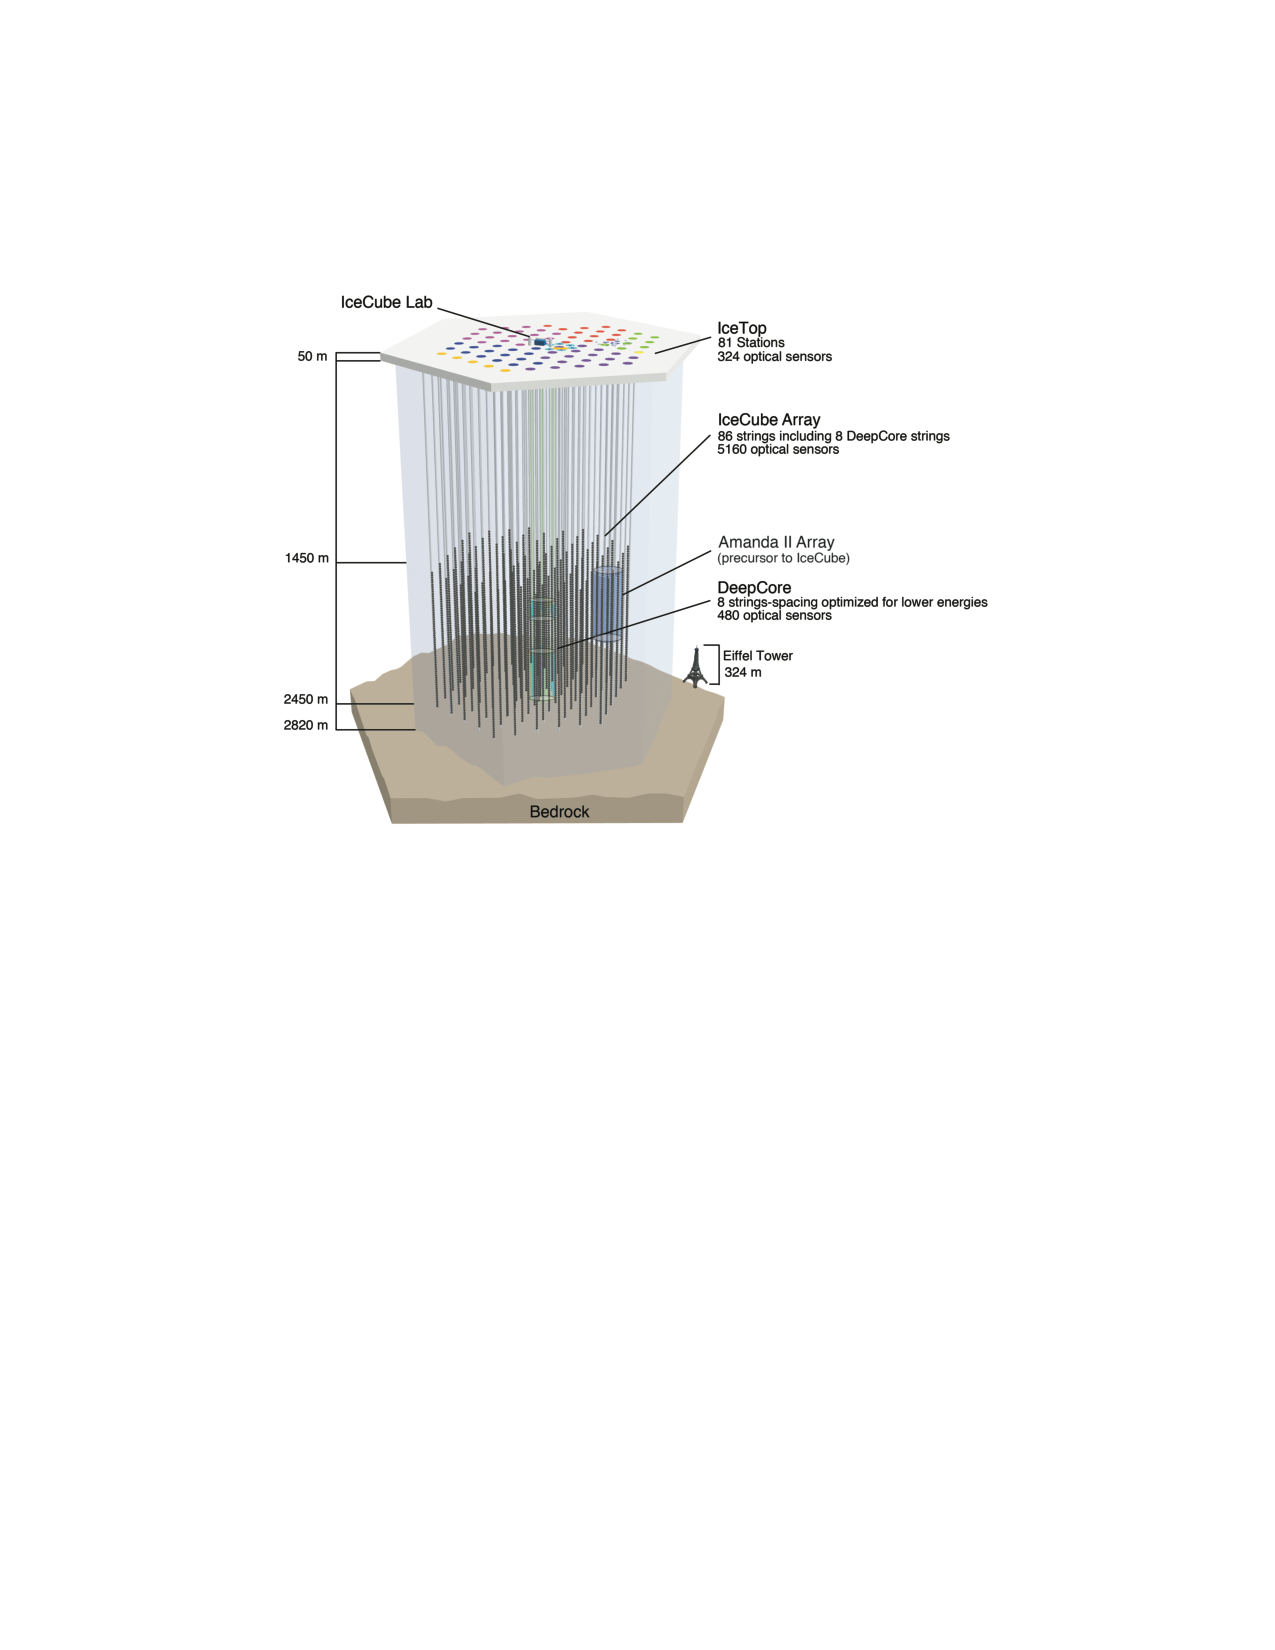
\includegraphics[width=0.8\textwidth]{./Icecube.pdf}
\caption{}
\end{figure}


\begin{itemize}
\item[a)]{Read the wikipedia article on Cherenkov radiation:  \href{https://en.wikipedia.org/wiki/Cherenkov_radiation}{https://en.wikipedia.org/wiki/Cherenkov\_radiation}}
\item[b)]{
The scattering process $\bar{\nu}_\mu + p \rightarrow \mu^+ n $ at IceCube occurs in the frame in which the proton (in the nucleus of a water molecule) is at rest. 
Assuming that the anti-neutrino’s momentum is aligned along the +z axis, write the four-momentum of the anti-muon and the neutron in terms of the anti-neutrino energy $E_\nu$ the nucleon mass $m_N$x, and the scattering angle $\theta$. 
You can safely assume that the anti-neutrino and anti-muon are both massless and the proton and neutron have identical mass equal to mN. 
The scattering angle is the angle between the original anti-neutrino momentum and the anti-muon’s momentum.
}
\item[c)]{
Figure 2 is a plot from the IceCube experiment that shows the deposited energy into the experiment versus the declination angle of the anti-muon from high-energy neutrino scattering. 
This plot shows the 37 highest energy events recorded by IceCube. 
There are three fantastically high energy events observed above 1000 TeV (= 1 Peta-electron Volt) of deposited energy. 
The highest energy event is affectionately called “Big Bird,” while the second and third highest energy events are called “Bert” and “Ernie.” 
(Actually, all of the events on this plot are named after Muppets.)

If the Big Bird anti-muon deposited 2 PeV of energy in IceCube, then what is the corresponding largest and smallest energy that the initial anti-neutrino could have had?

\begin{figure}[h!]
\centering
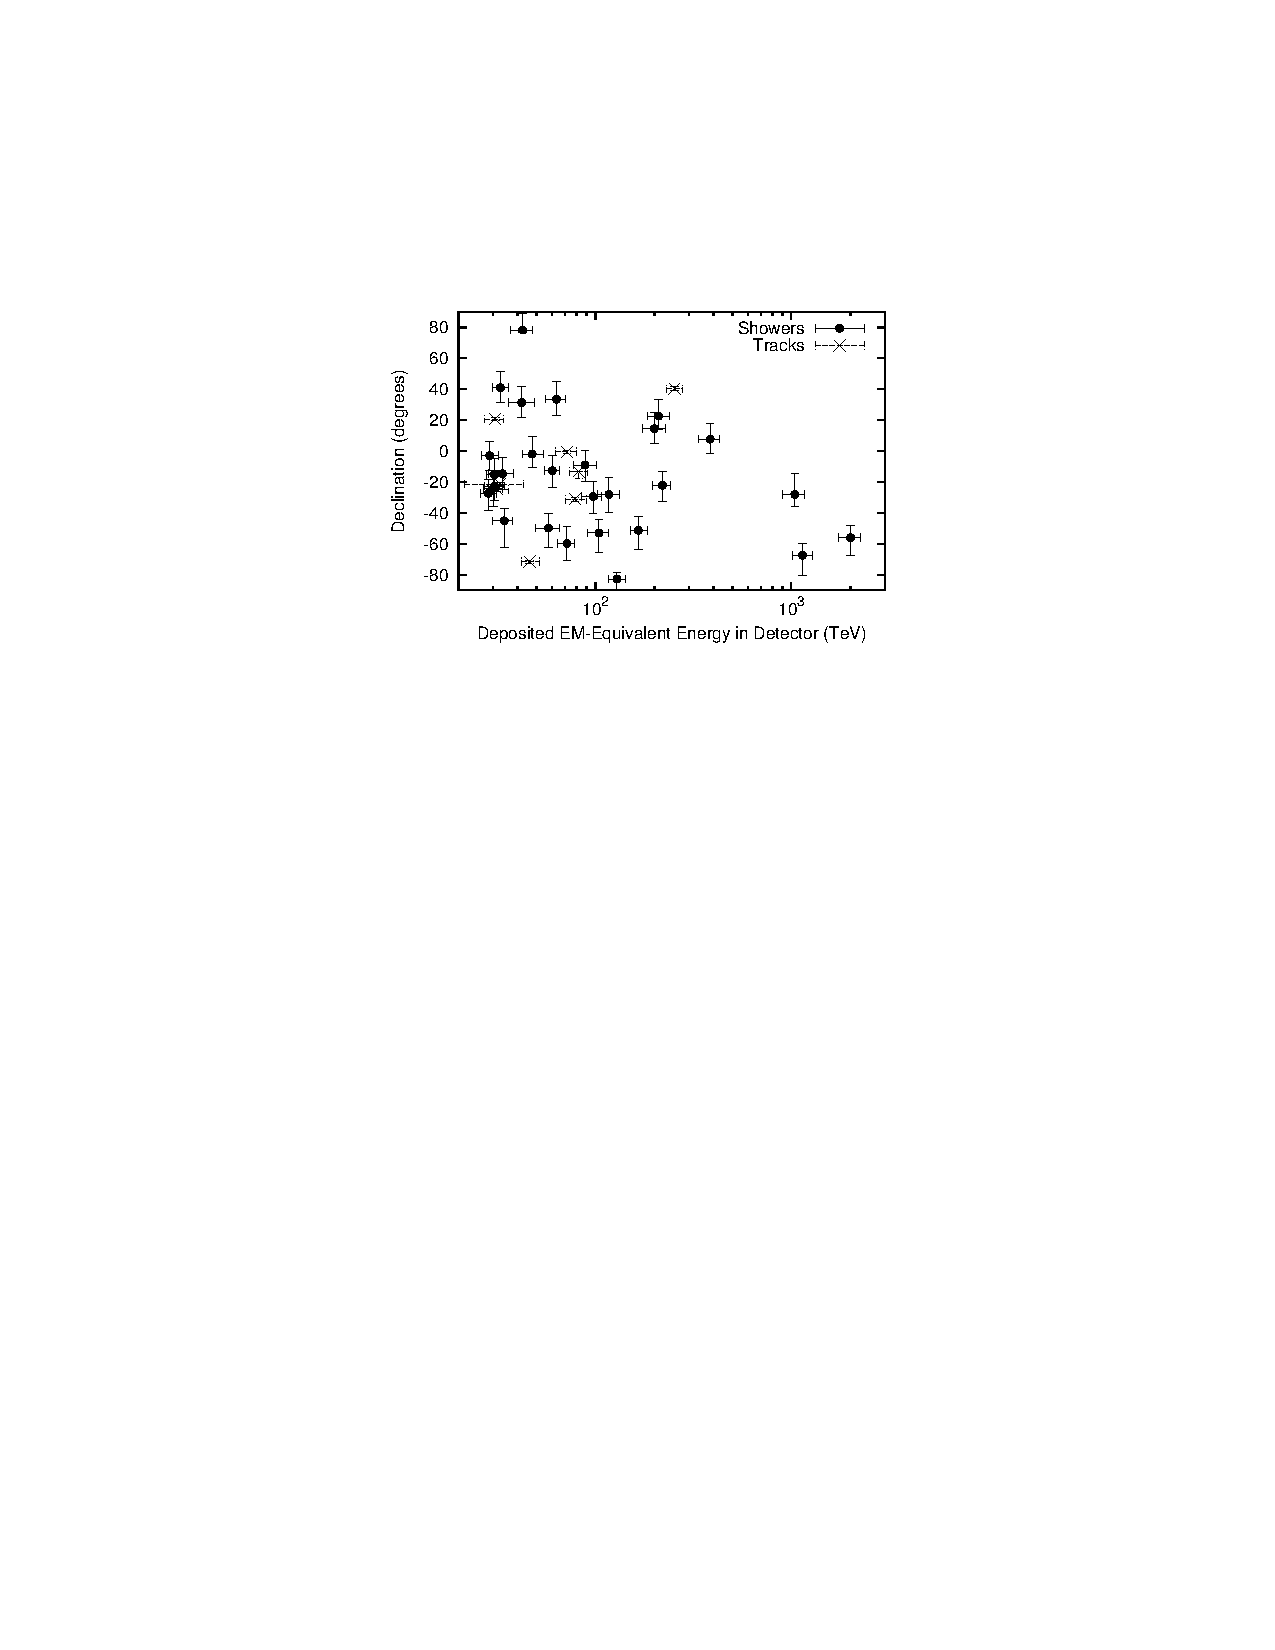
\includegraphics[width=0.8\textwidth]{./IcecubeData.pdf}
\caption{}
\end{figure}

}
\item[d)]{
What are the corresponding maximum and minimum scattering angles in degrees between the initial anti-neutrino and the measured Big Bird anti-muon? 
Call the maximum angle $\theta_{\mathrm{max}}$ and the minimum angle $\theta_{\mathrm{min}}$. 
For simplicity, set the mass of the proton/neutron to $m_N = 1$ GeV. 
With any possible anti-neutrino energy, is the momentum of the anti-muon close to the direction of the anti-neutrino? 
You can safely assume that $m_N << E_\mu$, so Taylor expanding would likely help.

\textit{This property of the scattering angle from part is extremely important for determining the astrophysical source of the high energy neutrinos observed in IceCube. 
In 2016, scientists on the Fermi Gamma Ray Space Telescope found evidence that the neutrino that was responsible for the Big Bird muon was created in a blazar, an enormously energetic radiation source believed to be generated by a supermassive black hole at the center of a galaxy.}
}
\item[e)]{Draw the Feynman diagram for $\bar{\nu}_\mu + p \rightarrow \mu^+ n $ assuming a point-like interaction and treating the proton and neutron as fundamental particles.}
\item[f)]{Use dimensional analysis to estimate the size of the $\bar{\nu}_\mu + p \rightarrow \mu^+ n $ cross section. \textit{Hint: The dependence on $E_\nu$ is very weak so express your answer only in terms of $m_p$ and $m_W$.}
}
\item[g)]{
IceCube ran for three years to find three events which each deposited more than a PeV of energy into the antarctic ice. 
Using the cross section above, approximately how many PeV neutrinos passed right through IceCube during that time? 
The total volume of the IceCube detector is about 1 km$^3$, and the density of ice is about 1000 $\frac{kg}{m^3}$.
}
\end{itemize}

Figure 3 is a display of the photomultiplier tube response in the Big Bird neutrino event. 
The strings on this figure correspond to the strings of photo-multiplier tubes, while the bubble region represents the detection of Cherenkov radiation.
 Larger bubbles corresponds to higher energies Cherenkov light detected. 

\begin{figure}[h!]
\centering
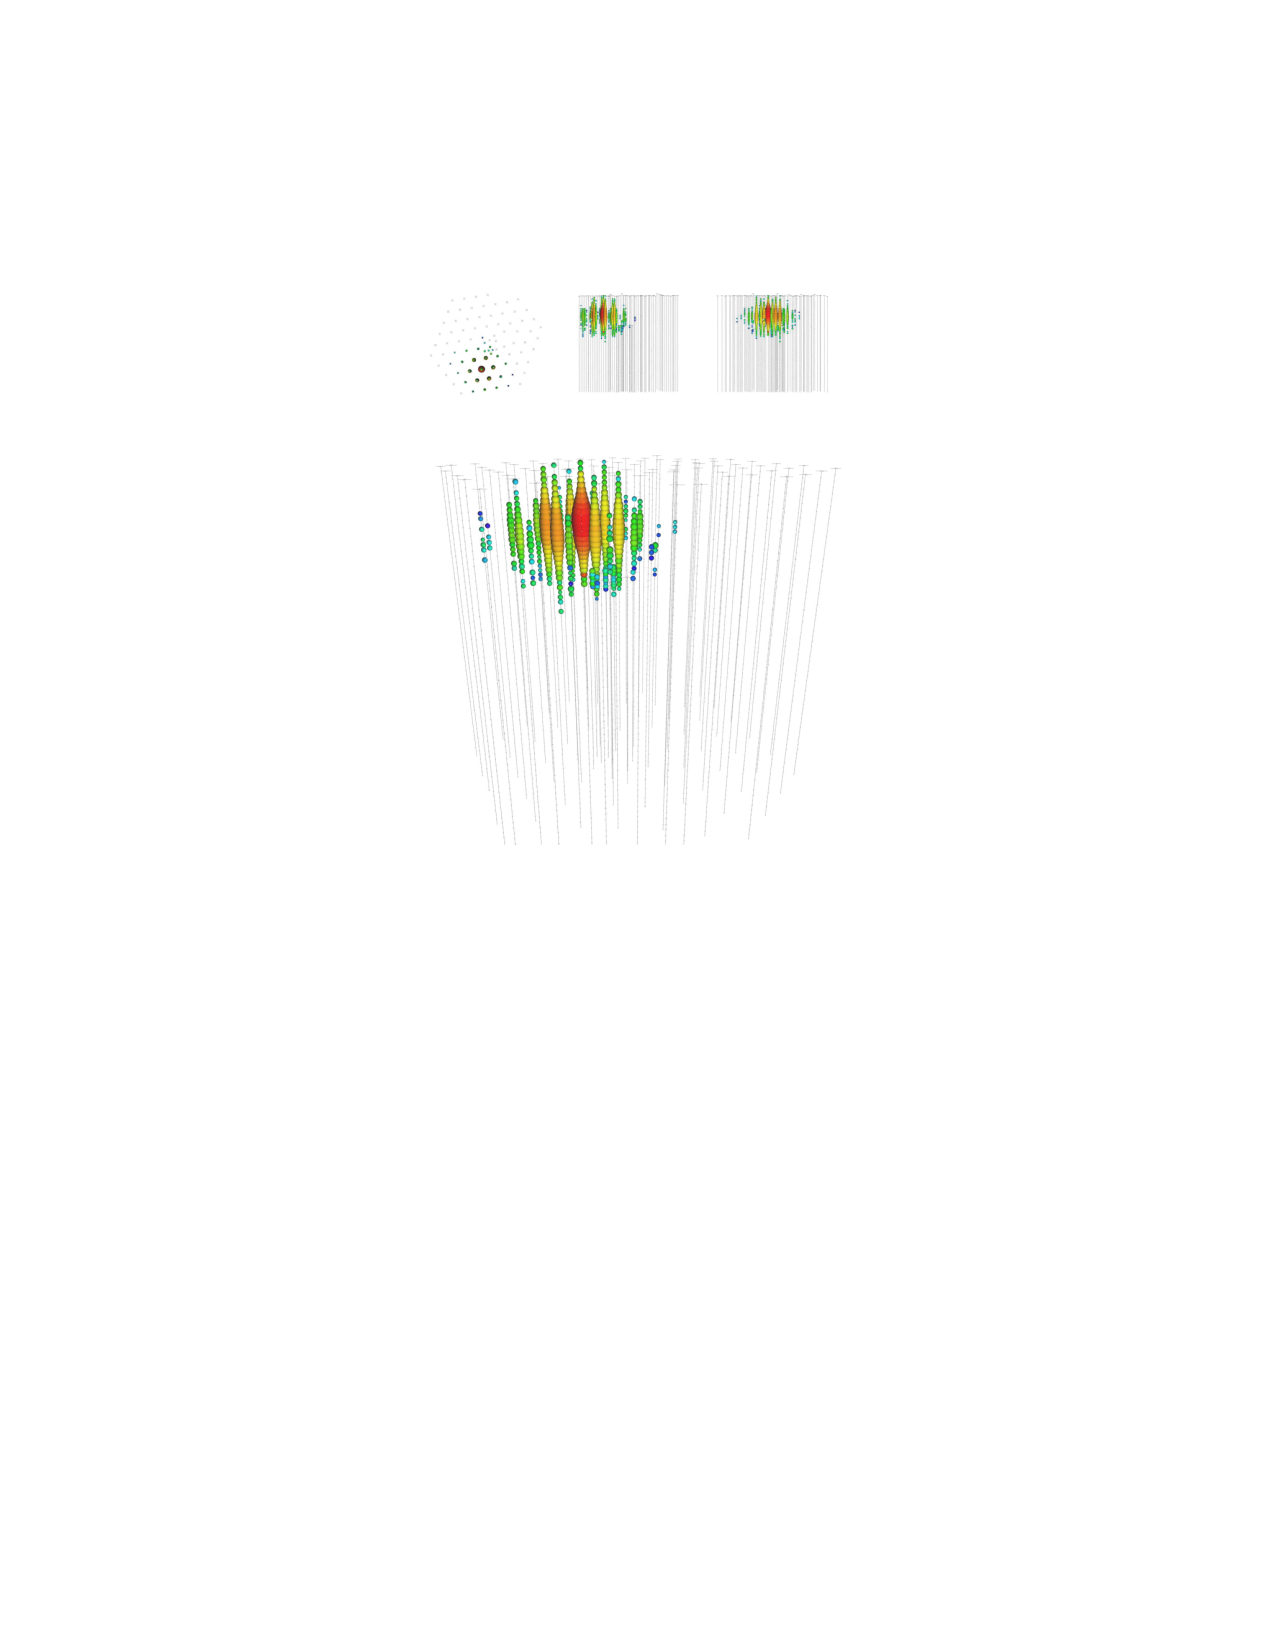
\includegraphics[width=0.8\textwidth]{./IceCubeBigBird.pdf}
\caption{}
\end{figure}


%\textbf{2) Tracking Detectors } \hfill \textit{(10 points)}\\
%
%Consider a charged particle emitted from a high-energy interaction, moving through a cylindrical tracking chamber of radius L under the influence of a solenoidal magnetic field B. 
%Assume that the particle moves in a plane perpendicular to the axis of the cylinder and the direction of the magnetic field.

%Because the initial direction of the particle is not a priori known, the curvature is measured from the sagitta s of its curved trajectory, defined to be the maximum deviation of the curve from a straight line between the point of origin and the point where the particle exits the detector at radius L.
%Show that, for small curvature, s = $\frac{qBL^2}{8p_T}$.}
%\item[b)]{
%If $\Delta s$ is the uncertainty in the measurement of the sagitta, derive the formula for $\frac{\Delta p_T}{p_T}$ in terms of $p_T$, L, B, and $\Delta s$.
%}
%\item[c)]{
%It can be shown that, if the tracking detector makes N equally spaced position measurement, each with resolution $\epsilon$, the uncertainty in the measurement of the sagitta is
%\be
%\Delta s = \frac{3.4 \epsilon }{\sqrt{N + 5}}
%\ee
%For N = 50, $\epsilon$ = 100 $\mu m$, L = 1 m, and B = 1 T, estimate the uncertainty in the obtained value of $p_T$.
%}
%\end{itemize}
%
%\vspace*{0.25in}
%
%\textbf{3) Limits of the Tracking System.} \hfill \textit{(5 points)}\\
%
%The tracking system at ATLAS is a cylinder with an outer radius of 1.1 meters which contains a 2 T solenoidal magnetic field, ie., the magnetic field lines are parallel to the axis of the cylinder. 
%Immediately outside of the tracking system is a region of 0 magnetic field, where the electromagnetic calorimeter is located.
%
%\begin{itemize}
%\item[a)]{
%The energy of charged particles that do not leave the tracking system is poorly measured because those particles do not reach the calorimetry. 
%Estimate the minimum $p_T$ in GeV for an electron to reach the calorimetry.
%}
%
%\item[b)]{
%The semiconductor tracker is a subsystem of the tracker that is also a cylinder, but with an outer radius radius of 0.5 meters. 
%It consists of layers of silicon that can measure particle positions accurate to 17 micrometers. 
%Extremely high energy charge particles do not bend enough in the magnetic field to have their charge accurately measured. 
%Estimate the maximum $p_T$ in GeV of a muon that the semiconductor tracker can determine bent in the magnetic field.
%}
%\item[c)]{
%For a high $p_T$ track that just bends in this magnetic field, what is the uncertainty in the measurement of the $p_T$? Estimate this using the resolution of the silicon tracking system.
%}
%\end{itemize}
%
%\vspace*{0.25in}
%
%\textbf{4) Rapidity.} \hfill \textit{(15 points)}\\
%
%\begin{itemize}
%\item[a)]{
%In experimental particle physics, it is often very useful to express the direction of motion of a particle in terms of its rapidity y. The rapidity is defined as
%\be
%y = \frac{1}{2} log \frac{E+p_z}{E - p_z}
%\ee
%for a particle with energy E and z-component of momentum $p_z$. 
%What makes rapidity so nice is its simple properties under Lorentz transformation. 
%Perform a Lorentz boost of the energy and momentum along the z-axis with velocity $\beta$. 
%How does the rapidity transform under this boost? 
%}
%\item[b.]{
%The pseudorapidity $\eta$ is defined as $\eta = - \ln \tan \frac{\theta}{2}$ where the polar angle is $\theta$ from the beam axis.
%Pseudorapidity is 0 for particles moving directly perpendicular to the beam at the interaction point. It is $\pm \infty$ along the proton beams where the polar angle is $0$ or $\pi$. 
%For a mass-less particle,  the polar angle is$\ \cos \theta = p_z/E$.
%How does rapidity y depend on pseudorapidity $\eta$ for mass-less particles?
%Any massless four-vector p can be expressed in $(\eta, \phi, p_T)$ coordinates as $p = p_T(\cosh \eta, \cos \phi,  \sin \phi, \sinh \eta)$
%}
%\item[c.]{
%
%The Figure is an event display from the ATLAS experiment. 
%The large image is a head-on view of the ATLAS experiment, with the tracker, calorimeters, and muon system visible. 
%At the lower right, is a so-called “Lego plot.” 
%This “unrolls” the detector, and displays the distribution of $p_T$ deposited in the $(\eta, \phi)$ plane.
%
%\begin{figure}[h!]
%\centering
%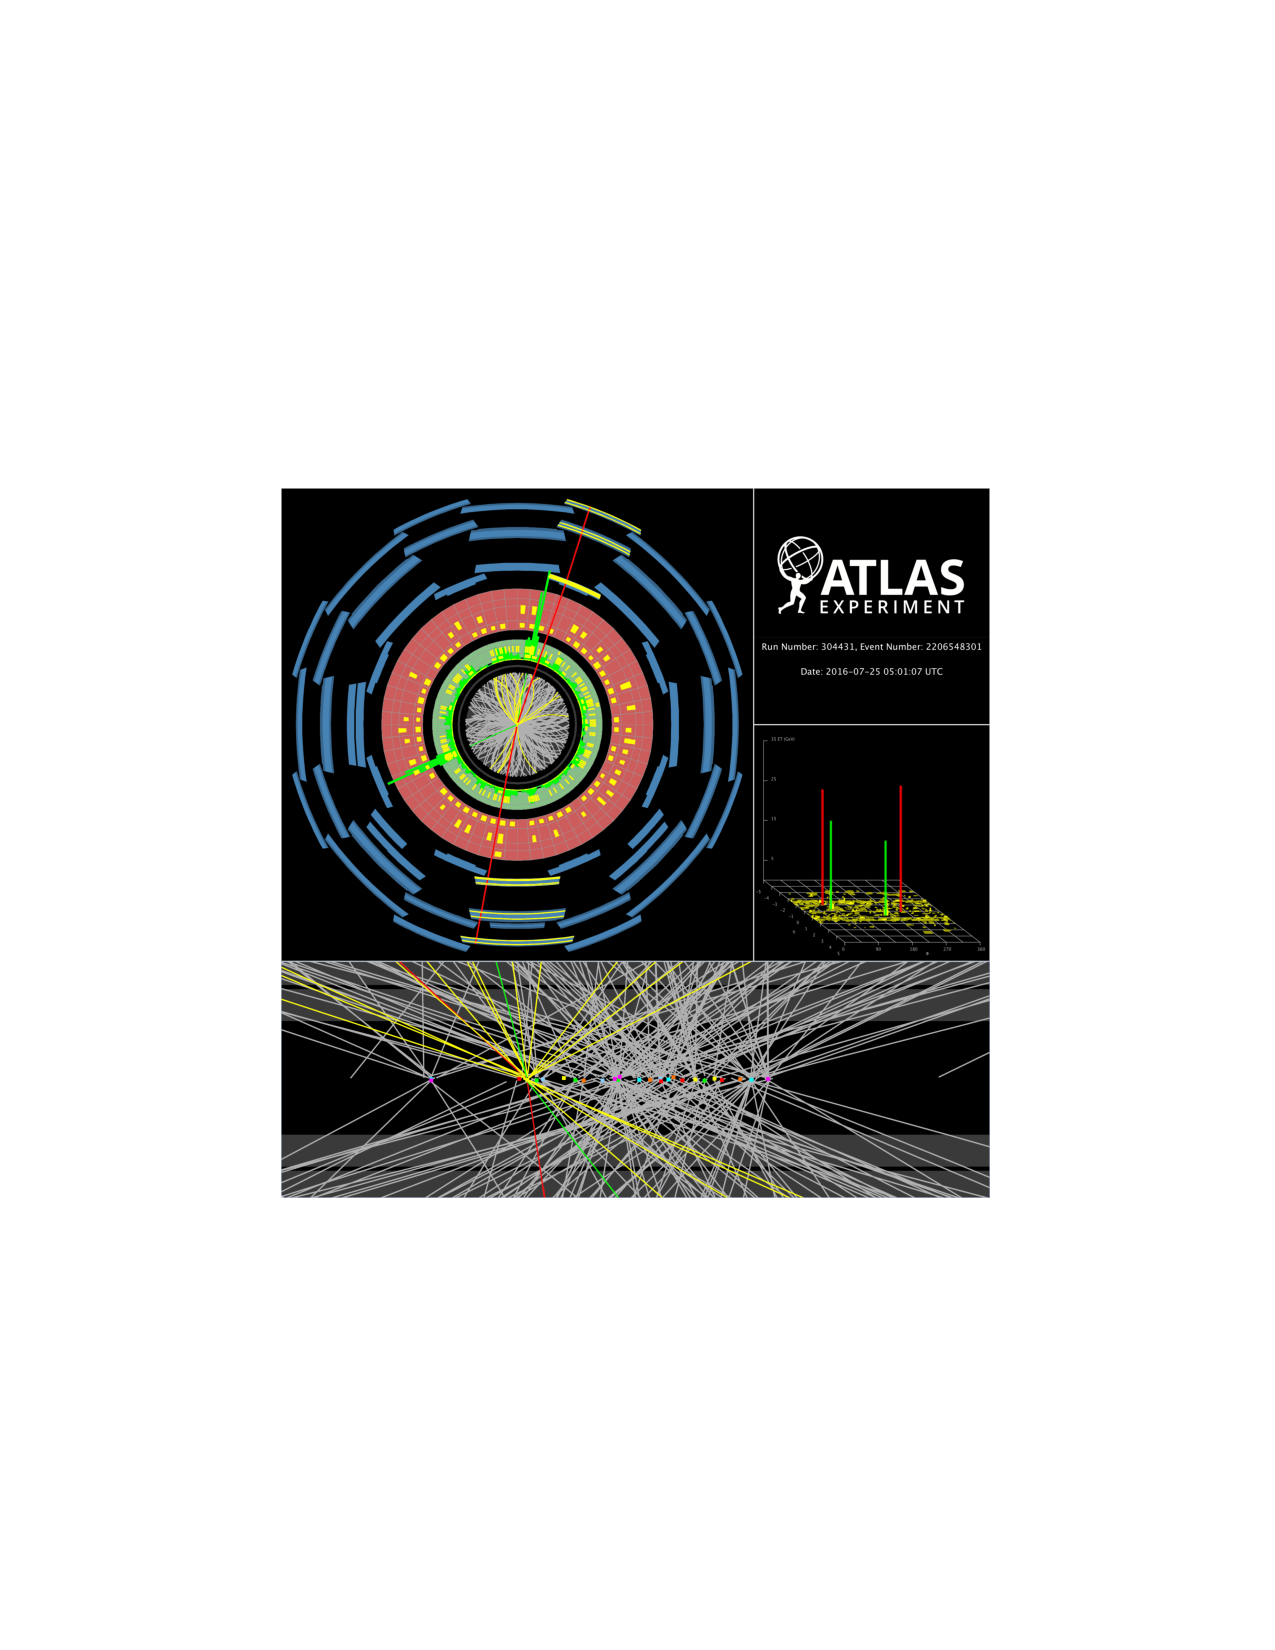
\includegraphics[width=0.8\textwidth]{./EventDisplay.pdf}
%\end{figure}
%
%\item[d.]{ Based on the “hits” in the tracker, EM calorimeter, hadronic calorimeter, and muon system, identify the particle type of the red and green spike in the Lego plot. 
%Both red particles are identical as are both green particles.}
%\item[e.]{
%From the Lego plot, determine the four-vectors of each of the red and green particles. 
%A zoomed in view of the Lego plot is also provided. You can safely neglect the particles’ masses. 
%}
%\item[f.]{
%What is the total transverse momentum vector of the four particles?
%}
%\item[h.]{What is the invariant mass of red particles together? Which particle of the Standard Model does this mass correspond most closely to?}
%\item[i.]{What is the invariant mass of green particles together? Which particle of the Standard Model does this mass correspond most closely to?}
%\item[j.]{What is the invariant mass of all particles together ? Which particle of the Standard Model does this mass correspond most closely to?}
%
%\begin{figure}[h!]
%\centering
%\includegraphics[width=0.8\textwidth]{./EventDisplayZoom.pdf}
%\end{figure}
%
%}
%
%
%\end{itemize}




}
\end{document}
